\chapter{تحكّم في الوقت !}

لهذا الفصل أهمية كبيرة : سيعلّمك كيف تتحكم في الوقت بالـ\textenglish{SDL}.
 إنه لمن النادر أن نقوم بإنشاء برنامج
\textenglish{SDL}
لا تحتاج إلى دوال خاصة بالتحكم في الوقت، بالرغم من أن لعبة
\textenglish{Mario Sokoban}
كانت حالة خاصة. رغم ذلك، في معظم الألعاب، إدارة الوقت هي شيء أساسيّ.

مثلاً، كيف لك أن تُنشئ لعبة 
\textenglish{Tetris}
أو
\textenglish{Snake} ؟
يجب فعلاً على الكُتل أن تتحرّك كل
\textenglish{X}
ثانية، و هذا ما لا تجيد فعله. على الأقل، قبل أن تقرأ هذا الفصل.

\section{الـ\textenglish{Delay} و الـ\textenglish{Ticks}}

في بادئ الأمر، سنتعلّم كيف نستعمل دالتين بسيطتين جداً :

\begin{itemize}
	\item \InlineCode{SDL\_Delay} :
	تسمح بتوقيف البرنامج مؤقتا لعدد من الميلّي ثواني.
	\item \InlineCode{SDL\_GetTicks} :
	تقوم بإرجاع عدد الميلّي ثواني التي مضت منذ انطلاق تشغيل البرنامج.
\end{itemize}

هاتان الدالّتان سهلتان جداً كما سنرى لكنّ استعمالهما ليس بسيطاً كما يبدو الأمر عليه.

\subsection{\texttt{SDL\_Delay}}

كما قلتُ، تقوم هذه الدالة بإيقاف عمل البرنامج لمدّة محدّدة. حينما يكون البرنامج متوقّفا، نقول أنّه "ينام" 
(\textenglish{sleep}) :
 هو لا يستعمل المُعالج. 
 
 يمكن إذا استعمال 
\InlineCode{SDL\_Delay}
للإنقاص من زمن اشتغال المُعالج 
(\textenglish{Processor}).
لاحظ أنّني سأختصره إلى 
\textenglish{CPU}
و هذا الإختصار متداول و يوافق العبارة 
"\textit{\textenglish{Central Processing Unit}}"
و الّتي تعني "وحدة المعالجة المركزيّة".\\
بفضل الـ\InlineCode{SDL\_Delay}
يمكنك جعل برامجك أقلّ شراهة لموارد المعالج. أي أننا لن نثقل على الحاسوب كثيراً إذا تمّ استخدام هذه الدالة بذكاء.

\begin{information}
هذا كلّه يعتمد على البرنامج الذي تـُنشئه : أحياناً، نجد أنه من المستحسن أن يستعمل البرنامج المعالج بشكل أقلّ، يمكن في نفس الوقت أن يقوم المُستعمل بشيء آخر مثلما هو الحال بالنسبة لقارئ
\textenglish{MP3}
الذي يشتغل في الخلفية ريثما تقوم بالتصفّح عبر الإنترنت.\\
لكن أحياناً، نحتاج للبرنامج أن يستعمل المعالج بنسبة 100\%، و هو الحال بالنسبة لغالبية الألعاب.
\end{information}

لنعد إلى الدالة، هذا نموذجها و هو بسيط للغاية :

\begin{Csource}
void SDL_Delay(Uint32 ms);
\end{Csource}

الأمر واضح، تبعث للدالة عدد الميلّي ثواني التي يجب أن "ينام" البرنامج خلالها. 

مثلاً : إذا أردت أن ينام البرنامج لمدّة ثانية واحدة، يجب عليك كتابة :

\begin{Csource}
SDL_Delay(1000);
\end{Csource}

 
لا تنس أنّها بالميلي ثانية :

\begin{itemize}
	\item 1000 ميلّي ثانية = ثانية.
	\item 500 ميلّي ثانية = نصف ثانية.
	\item 250 ميلّي ثانية = رُبع ثانية.
\end{itemize}

\begin{warning}
لا يمكنك فعل أي شيء في البرنامج بينما هو متوقّف مؤقّتا ! فالبرنامج "النائم" لا يمكن له فعل أي شيء لأنه ليس مفعّلا بالنسبة للحاسوب.
\end{warning}

\subsubsection{مشكل جزئيّة الوقت}

لا، تأكّد بأنني لن أخوض في درس للفيزياء الكميّة في هذا الفصل حول الـ\textenglish{SDL} !
و مع ذلك، أرى بأن هناك أمورا يجب عليك معرفتها : 
\InlineCode{SDL\_Delay}
ليست دالة "مثالية". و هذا ليس خطأها، بل هو خطأ نظام التشغيل 
(\textenglish{Windows}، \mbox{\textenglish{GNU/Linux}}، \mbox{\textenglish{Mac OS X}} \dots).

لماذا يتدخّل نظام التشغيل هنا ؟ ببساطة لأنه هو الذي يتحكّم في البرامج المشغّلة ! فبرنامجك سيقول للنظام : "سأنام، أيقظني بعد ثانية". لكن لن يقوم النظام دائما بإفاقة البرنامج بعد ثانية بالضبط.

في الواقع، قد يكون هناك تأخّر بسيط (تأخر 10 ميلّي ثانية بالتقريب كمعدّل، هذا يختلف حسب الحاسوب). لماذا ؟ لأن
\textenglish{CPU}
لا يمكنه العمل إلا على برنامج واحد في المرّة الواحدة. دور نظام التشغيل يتمثّل في إخبار
\textenglish{CPU}
بخصوص ما يجب أن يتم القيام به و لهذا : "لمدّة 40 ميلّي ثانية ستعملُ على
\InlineCode{firefox.exe}
ثم لمدّة 110 ميلّي ثانية على 
\InlineCode{explorer.exe}،
بعد ذلك، لمدة 80 ميلّي ثانية ستعمل على
\InlineCode{program\_sdl.exe}
ثم عد إلى العمل على
\InlineCode{firefox.exe}
لمدّة 65 ميلّي ثانية
\dots"
نظام التشغيل هو بالفعل عبارة عن قائد الأوركسترا~!

تخيّل الآن أنه لثانية من الزمن، يكون برنامج آخر لازال في طور الإشتغال : يجب أن ينتهي عمله حتى يستطيع برنامجك "استعادة التحكّم" على
\textenglish{CPU}.

ما الذي يجب تذكّره ؟ أن
\textenglish{CPU}
لا يمكنه أن يتحكّم في برنامجين في آن واحد. و لكي يعطي انطباعاً بأنه يُشغّل العديد من البرامج في نفس اللحظة، يقوم بتقسيم الوقت بين هذه البرامج حيث تعملُ دوراً بدور.\\
قَلَّت صحّة هذا الكلام لأن المعالجات "ثنائية النوى" لها القدرة على تشغيل برنامجين في نفس الآن. 

لكن هذه التقنية في التحكّم بالبرامج معقّدة للغاية و لن نحصل على ضمانات بأنّ البرنامج الخاص بنا سيتمّ إيقاظة في ثانية بالضبط من الزمن.

مع ذلك، يعتمد الأمر دائماً على الحاسوب نفسه كما قلتُ سابقاً. عندي، ألاحظ أنّ الدالّة
\InlineCode{SDL\_Delay}
دقيقة جدّا.
\begin{information}
 بسبب مشكل جزئيّة الوقت، لن تتمكّن إذا من إيقاف برنامجك مؤقّتا لوقت قصير جدّا من الزمن، أي أنه لو استعملت 
\InlineCode{SDL\_Delay(1);}
ستكون متأكداً بأن البرنامج لن ينام لـ1 ميلي ثانية و إنما أكثر (حوالي 9 أو 10 ميلي ثانية).
\end{information}

الدالة
\InlineCode{SDL\_Delay}
عمليّة، لكن لا تثق بها كثيراً. فهي لا توقف البرنامج بالمقدار الزمني الذي تحدده أنت بالضبط. \\
هذا ليس راجعاً لكون الدالة غير مُبرمجة جيداً، لكن لأن عمل الجهاز معقّد و لا يمكنه أن يكون دقيقاً من هذه الناحية.

\subsection{\texttt{SDL\_GetTicks}}

هذه الدالة تُرجع عدد الميلي ثواني التي انقضت منذ بدأ عمل البرنامج. و هي عبارة عن مؤشّر للزمن لا يمكن الاستغناء عنه. ستجد بأنها مفيدة لكي تضع مراجع في الزمن، سترى ذلك !

هذا نموذجها :

\begin{Csource}
Uint32 SDL_GetTicks(void);
\end{Csource}

هذه الدالة لا تنتظر أي معامل، و هي تقوم فقط بإرجاع عدد الثواني المنقضية. \\
هذا العدد يتصاعد مع مضي الزمن. لمعلوماتك، التوثيق الخاص بالـ\textenglish{SDL}
يشير إلى أن هذا العدد يصل إلى الحد الأقصى 49 يوما ثم يبدأ العدد من جديد ! لكن يجدر بالبرنامج الذي تكتبه ألا يستمرّ كلّ هذا الوقت و لهذا فلا تقلق من هذه الناحية.

\subsection{إستعمال \texttt{SDL\_GetTicks} لإدارة الوقت}

إذا كانت الدالة
\InlineCode{SDL\_Delay}
سهلة للفهم و للاسعمال، فالأمر ليس عينه بالنسبة لـ\InlineCode{SDL\_GetTicks}.
حان الوقت لنعرف كيف سنستفيد منها.\\
إليك هذا المثال، سنسترجع البرنامج القديم الذي يقوم بإظهار نافدة تحتوي على
\textenglish{Zozor}
(الصورة التالية) :

\begin{figure}[H]
	\centering
	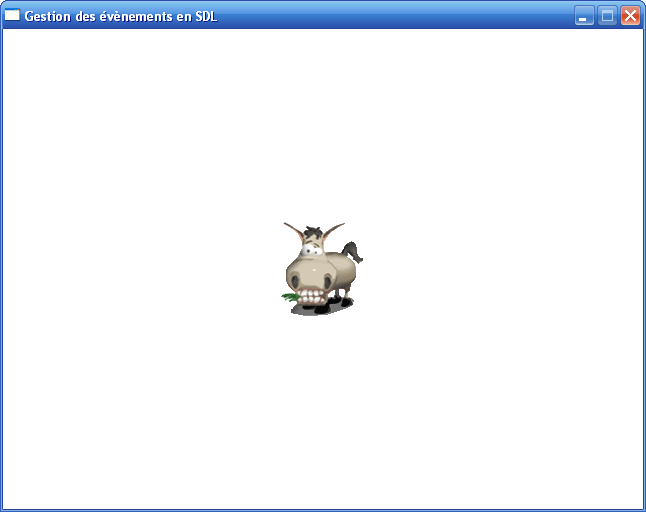
\includegraphics[width=0.8\textwidth]{Chapter_III-4_Window-Zozor}
\end{figure}

هذه المرة، في عوض التحكّم في حركة
\textenglish{Zozor}
بالفأرة أو بلوحة المفاتيح، سنعتمد فكرة أنه سيقوم بالتحرّك لوحده في الشاشة. لبنسّط الأمور، سنجعله يتحرّك أفقيا في النافذة. 

سنُعيد استعمال نفس الشفرة التي استخدمناها في فصل الأحداث، يجدر بك أن تجيد كتابتها بنفسك دون الحاجة لمُساعدة مني. و إلا،  إذا احتجتها، يمكنك استعادتها من الفصول السابقة.

\begin{Csource}
int main(int argc, char *argv[])
{
	SDL_Surface *screen = NULL, *zozor = NULL;
	SDL_Rect zozorPosition;
	SDL_Event event;
	int cont = 1;
	SDL_Init(SDL_INIT_VIDEO);
	screen = SDL_SetVideoMode(640, 480, 32, SDL_HWSURFACE | SDL_DOUBLEBUF);
	SDL_WM_SetCaption("Gestion du temps en SDL", NULL);
	zozor = SDL_LoadBMP("zozor.bmp");
	SDL_SetColorKey(zozor, SDL_SRCCOLORKEY, SDL_MapRGB(zozor->format, 0, 0, 255));
	zozorPosition.x = screen->w / 2 - zozor->w / 2;
	zozorPosition.y = screen->h / 2 - zozor->h / 2;
	SDL_EnableKeyRepeat(10, 10);
	while (cont)
	{
		SDL_WaitEvent(&event);
		switch(event.type)
		{
			case SDL_QUIT:
			cont = 0;
			break;
		}
		SDL_FillRect(screen, NULL, SDL_MapRGB(screen->format, 255, 255, 255));
		SDL_BlitSurface(zozor, NULL, screen, &zozorPosition);
		SDL_Flip(screen);
	}
	SDL_FreeSurface(zozor);
	SDL_Quit();
	return EXIT_SUCCESS;
}
\end{Csource}

فلنهتم بـ\textenglish{Zozor}.
نريد أن نحرّكه. من أجل هذا، سيكون من الأفضل استعمال 
\InlineCode{SDL\_GetTicks}.
سنحتاج إلى متغيرين : 
\InlineCode{previousTime}
و 
\InlineCode{currentTime}.
يستخدمان من أجل تخزين الوقت الذي تمّ إرجاعه من طرف 
\InlineCode{SDL\_GetTicks}
في لحظات زمنية مختلفة.\\
يكفي أن نحسب الفرق بين 
\InlineCode{currentTime}
و
\InlineCode{previousTime}
لمعرفة الوقت المنقضّي. إذا كان هذا الأخير يساوي 30 ميلي ثانية، نغيّر إحداثيات 
\textenglish{Zozor}.

لنبدأ إذا بإنشاء هذين المتغيرين  :

\begin{Csource}
int previousTime = 0, currentTime = 0;
\end{Csource}

و الآن، في حلقتنا غير المنتهية، نضيف الشفرة المصدرية التالية :

\begin{Csource}
currentTime = SDL_GetTicks();
if (currentTime - previousTime > 30) // If 30 ms have passed
{
	zozorPosition.x++; // We move Zozor
	previousTime = currentTime; // The current time becomes the previous one.
}
\end{Csource}

اِفهم جيّدا ما يحصل :

\begin{enumerate}
	\item نحصل على الوقت المنقضي باستعمال
	\InlineCode{SDL\_GetTicks}.
	\item نقارن هذه القيمة بالوقت الذي تم تسجيله مسبقاً. إذا كان هناك فرق 30 مث على الأقل، إذا\dots
	\item نحرّك
	\textenglish{Zozor}،
	لأننا نريده أن يتحرّك كلّ 30 مث. هنا، نقوم بتحريكه إلى اليمين كلّ 30 مث. \\
	يجب ان نتأكد ما إن كان الوقت المنقضي أكبر من 30 مث، و ليس ما إن كان يساوي تلك القيمة~! لأنه في الواقع سنُخْبَر ما إن كان الوقت المنقضي يساوي على الأقل 30 مث. نحن لسنا متأكدين بأنه سيتمّ تنفيذ الأمر كلّ 30 مث بالضبط.
	\item ثم، و الأمر الذي لا يجب فعلاً نسيانه، نضع قيمة الوقت "الحالي" في الوقت "السابق". بالفعل، تخيّل الدورة القادمة للحلقة : الوقت الحالي يتغيّر و يمكننا مقارنته بالوقت السابق من جديد، أي سنقارن ما إن تم انقضاء 30 مث على الأقل ثم نحرّك
	\textenglish{Zozor}.
\end{enumerate}

\begin{question}
و لكن ماذا يحصل لو أن الحلقة اشتغلت لمدّة أقل من 30 مث ؟
\end{question}

اِقرأ جيداً الشفرة، لا شيء سيحدث !\\
لن ندخل في الشرط، يعني أننا لن نقوم بأي شيء. ننتظر الدورة القادمة للحلقة أين نقوم من جديد باختبار ما إن تم انقضاء 30 مث منذ آخر مرّة قمنا فيها بتحريك 
\textenglish{Zozor}.

هذه الشفرة قصيرة، لكن يجب فهمها ! أعد قراءة شرحي بالعدد اللازم من المرّات لتفهم جيداً لأن هذا الجزء قد يكون الأهم في هذا الفصل.

\subsubsection{تغيير في معالجة بالأحداث}

الشفرة المصدرية الذي كتبناها مثالية إلى حدّ ما إذ ينقصها تفصيل بسيط : الدالة 
\InlineCode{SDL\_WaitEvent}.
كانت هذه الدالة عمليّة إلى حدّ الآن بما أننا لم نتحكّم في الوقت. هذه الدالة توقف البرنامج مؤقّتا (بنفس طريقة
\InlineCode{SDL\_Delay}
تقريباً) ما دام لا يوجد أي حدث.

لكن هنا، لسنا مُضطرين إلى انتظار حدث لنقوم بتحريك
\textenglish{Zozor} !
إذ يجب عليه التحرّك لوحده.\\
و لا يجب عليك الاستمرار في تحريك الفأرة فقط لإنتاج أحداث و منه الخروج من الدالة 
\InlineCode{SDL\_WaitEvent}~!

ماهو الحلّ ؟ 
\InlineCode{SDL\_PollEvent}.\\
لقد قدّمت لك من قبل هذه الدالة : على عكس
\InlineCode{SDL\_WaitEvent}،
تُرجع هذه الدالة قيمة سواء كان هناك حدث أم لا. و نقول بأن الدالة غير مـُعطّـِلة : هي لا توقف البرنامج مؤقّتا لأن الحلقة غير المنتهية ستستمرّ في العمل طوال الوقت.

\subsubsection{الشفرة المصدرية الكاملة}

هذه هي الشفرة النهائية التي بإمكانك تجريبها :

\begin{Csource}
int main(int argc, char *argv[])
{
	SDL_Surface *screen = NULL, *zozor = NULL;
	SDL_Rect zozorPosition;
	SDL_Event event;
	int cont = 1;
	int previousTime = 0, currentTime = 0;
	SDL_Init(SDL_INIT_VIDEO);
	screen = SDL_SetVideoMode(640, 480, 32, SDL_HWSURFACE | SDL_DOUBLEBUF);
	SDL_WM_SetCaption("Gestion du temps en SDL", NULL);
	zozor = SDL_LoadBMP("zozor.bmp");
	SDL_SetColorKey(zozor,SDL_SRCCOLORKEY, SDL_MapRGB(zozor->format, 0, 0, 255));
	zozorPosition.x = screen->w / 2 - zozor->w / 2;
	zozorPosition.y = screen->h / 2 - zozor->h / 2;
	SDL_EnableKeyRepeat(10, 10);
	while (cont)
	{
		SDL_PollEvent(&event); // We use PollEvent and not WaitEvent in order not to block the program
		switch(event.type)
		{
			case SDL_QUIT:
			cont = 0;
			break;
		}
		currentTime = SDL_GetTicks();
		if (currentTime - previousTime > 30) // If 30ms have passed since the final loop iteration
		{
			zozorPosition.x++; // We move Zozor
			previousTime = currentTime; // The current time becomes the previous one for our future calculation.
		}
		SDL_FillRect(screen, NULL, SDL_MapRGB(screen->format, 255, 255, 255));
		SDL_BlitSurface(zozor, NULL, screen, &zozorPosition);
		SDL_Flip(screen);
	}
	SDL_FreeSurface(zozor);
	SDL_Quit();
	return EXIT_SUCCESS;
}
\end{Csource}

يجدُر بك أن ترى
\textenglish{Zozor}
يهتزّ لوحده على الشاشة. هو يتحرّك نحو اليمين. \\
حاول مثلاً تغيير الوقت من 30 مث إلى 15 مث : يجدر بـ\textenglish{Zozor}
أن يتحرّك إلى اليمين بشكل أسرع بمرتين ! في الواقع، هو يتحرّك مرّة كل 15 مث في عوض مرّة كل 30 مث كالسابق.

\subsubsection{استهلاك أقل للـ\textenglish{CPU}}

حالياً، البرنامج يدور في حلقة غير منتهية بسرعة الضوء (حسنا، تقريباً). و لهذا فهو يستهلك 100\% من المعالج. لكي نرى هذا يكفي مثلاُ أن نضغط على 
\InlineCode{CTRL} + \InlineCode{ALT} + \InlineCode{DEL}
(في القائمة
\textenglish{Processes})
في
\textenglish{Windows} :

\begin{figure}[H]
	\centering
	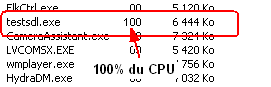
\includegraphics[width=0.4\textwidth]{Chapter_III-6_Process}
\end{figure}

كما يمكنك أن ترى، يتم استعمال
\textenglish{CPU}
بنسبة 100\% من طرف برنامجنا
\InlineCode{testsdl.exe}.\\
لقد قلت لك مسبّقاً : إذا برمجت لعبة (خاصة إذا كانت بنظام شاشة كاملة)، ليس خطيراً أن تستعمل المعالج بنسبة 100\%. لكن إذا كانت لعبة في نافذة مثلاً، يُستحسن استعمال نسبة أقل من
\textenglish{CPU}
لكي نسمح للمستعمل بالقيام بشيء آخر دون أن يُجهد الحاسوب نفسه.

الحل ؟ سنقوم بإعادة الشفرة السابقة، لكننا سنضيف إليه
\InlineCode{SDL\_Delay}
من أجل انتظار الوقت اللازم لكي يصل إلى 30 مث.

يكفي أن نضيف
\InlineCode{SDL\_Delay}
في 
\InlineCode{else} :

\begin{Csource}
currentTime = SDL_GetTicks();
if (currentTime - previousTime > 30) // If 30ms have passed
{
	zozorPosition.x++; // We move Zozor
	previousTime = currentTime; // The current time becomes the previous one for our future calculation
}
else
{
	SDL_Delay(30 - (currentTime - previousTime));
}
\end{Csource}

كيف تعمل الأمور هذه المرة ؟ الأمر بسيط، هناك احتمالان (حسب الشرط) :

\begin{itemize}
	\item إما أنه مضت اكثر من 30 مث منذ قمنا بتحريك
	\textenglish{Zozor}،
	في هذه الحالة نحرّكه.
	\item إما أنه مضى وقت أقل من 30 مث، في هذه الحالة سينام البرنامج بفضل
	\InlineCode{SDL\_Delay}
	ريثما يسمح بوصول الـ30 مث و بهذه العملية الحسابية التي قمتُ بها
	\InlineCode{30 - (currentTime - previousTime)}.
	إذا كان الفرق بين الزمن الحالي و الزمن السابق هي 20 مث مثلاً، فسينام البرنامج لـ
	30 - 20 = 10
	مث لكي تصل الـ30 مث.
\end{itemize}

\begin{information}
تذكّر بأن
\InlineCode{SDL\_Delay}
يمكن لها أن تضيف بعض الميلّي ثواني أكثر من المتوقع.
\end{information}

بهذه الشفرة، سينام البرنامج معظم الوقت و بهذا نقلل من استهلاك
\textenglish{CPU}.
لاحظ الصورة التالية :

\begin{figure}[H]
	\centering
	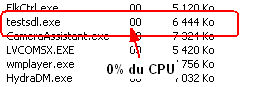
\includegraphics[width=0.4\textwidth]{Chapter_III-6_Process-0}
\end{figure}

يستعمل البرنامج كمعدّل حوالي 0 إلى 1\% من 
\textenglish{CPU}\dots
أحياناً يستعمل أكثر بقليل لكنّه يعود سريعاً إلى 0\%.

\subsubsection{التحكّم في عدد الصور في الثانية}

أنت تتساءل حتماً كيف يمكننا الحدّ من (أو تثبيت) عدد الصور في الثانية (غالباً ما نسمّي هذا
\textenglish{FPS}
اِختصاراً لـ\textenglish{Frames per second})
التي يُظهرها الحاسوب.

حسناً، هذا تماماً ما نحاول فعله ! فهنا نقوم بإظهار صورة جديدة كل 30 مث كمعدّل. علماً أن ثانية واحدة تساوي 1000 مث، لكي نجد عدد الـ\textenglish{FPS}،
يجب أن نقوم بعملية قسمة
1000 / 30 = 33
 صورة في الثانية بالتقريب.
 
بالنسبة لعين الإنسان، نقول عن التحرّك أنه رشيق إذا احتوى على الأقل 25 صورة في الثانية. بـ33 صورة في الثانية إذاً فالتحرّك في البرنامج رشيق تماما و بهذا لن يظهر متشنّجا. 

إذا أردنا صورا أكثر في الثانية، يجب إنقاص حدود الوقت بين صورتين. انتقل من 30 إلى 20 مث و ستصبح العملية :
1000 / 20 = 50 \textenglish{FPS}.

\subsubsection{تمارين}
التحكّم في الوقت ليس أمراً بديهياً، سيكون من الجيد لك أن تتمرّن، ما رأيك ؟ إليك بعض التمارين :

\begin{itemize}
	\item  لحدّ الآن، يتحرّك 
	\textenglish{Zozor}
	في كلّ مرة إلى اليمين إلى أن يختفي من الشاشة. سيكون من الأفضل حينما يصل إلى حافة النافذة أن يعيد التوجّه إلى اليسار. سيكون ذلك أفضل أليس كذلك ؟ لأنه سيعطي انطباعاً أنه يرتدّ.
	
	أنصحك بإنشاء متغير منطقي
	\InlineCode{toTheRight}
	يحمل القيمة "صحيح" إذا كان 
	\textenglish{Zozor}
	يتحرّك نحو اليمين (و "خطأ" إذا كان يتحرّك نحو اليسار). إذا كان المتغير المنطقي يحمل القيمة صحيح، تقوم بتحريك
	\textenglish{Zozor}
	إلى اليمين، و إلا فستقوم بتحريكه إلى اليسار. لا تنس أن تغيّر قيمة المتغير المنطقي ما إن يصل
	\textenglish{Zozor}
	إلى حافة النافذة و ذلك لكي ينطلق في الإتجاه المُعاكس !
	\item بدل أن يقوم 
	\textenglish{Zozor} 
	بالإرتداد من اليمين إلى اليسار، فيمكن تحريكه على قطر النافذة ! يكفيك تغيير 
	\InlineCode{zozorPosition.x}
	و 
	\InlineCode{zozorPosition.y}
	في نفس الوقت. يمكنك رؤية ماذا يُعطينا الأمر لو نقوم بزيادة قيمة 
	\InlineCode{x}
	و إنقاص قيمة 
	\InlineCode{y}
	في نفس الوقت، أو إذا قُمنا بزيادة قيمتيهما معاً، إلخ.
	\item حاول جعل
	\textenglish{Zozor}
	يتوقّف عن التحرّك إذا تمّ الضغط على الزر
	\InlineCode{P}،
	و إذا تم الضغط مجدداً على نفس الزر ينطلق
	\textenglish{Zozor}
	مجدداً. يحتاج الأمر متغيرا منطقيا بسيطا تقوم بتفعيله أو تعطيله.
\end{itemize}

\section{المُؤقـِتات (\textenglish{Timers})}

\begin{warning}
استعمال 
\textit{المُؤقـِتات}
أكثر تعقيداً قليلاً لأننا سنعتمد على مبدأ لم نره لحدّ الآن : المؤشّرات نحو الدوال. استعمال المُؤقـِتات ليس أمراً ضروريا : إذا وجدت بأنها صعبة جداً لتستعملها، يمكنك غضّ النظر عنها دون أي مشكل.
\end{warning}

المُؤقـِتات تشكّل طريقة أخرى لتحقيق ما نحن بصدد رؤيته بالدالة 
\InlineCode{SDL\_GetTicks}.\\
هي تقنية خاصّة نوعاً ما. بعض المبرمجين يجدونها عمليّة، و آخرون لا. هذا يعتمد على ذوقك البرمجي.

ماهو 
\textit{المُؤقـِت} ؟\\
هو نظام يسمح بالطلب من الـ\textenglish{SDL}
أن تستدعي دالة ما كل 
\textenglish{X}
ميلّي ثانية. يمكنك بهذا أن تنشئ دالة 
\InlineCode{moveEnemy()}
تقوم الـ\textenglish{SDL}
باستدعائها تلقائيّا كل 50 مث كي يستطيع العدوّ التحرّك في مجالات معيّنة.

\begin{information}
كما كنت أقول لك الآن، يمكننا القيام بهذا بواسطة
\InlineCode{SDL\_GetTicks}
باستعمال التقنية التي رأيناها أعلاه.\\
ما الفائدة إذا ؟ لنقل أن المُؤقـِتات تفرض علينا هيكلة برامجنا بشكل أفضل على شكل دوال.
\end{information}

\subsection{تهيئة نظام المُؤقـِتات}

لكي نتمكّن من استعمال المُؤقـِتات، يجب علينا تهيئة الـ\textenglish{SDL}
أولاً باستعمال عَـلَم خاص :
\InlineCode{SDL\_INIT\_TIMER}.
يجب عليك إذا استدعاء الدالة
\InlineCode{SDL\_Init}
كالتالي :

\begin{Csource}
SDL_Init(SDL_INIT_VIDEO | SDL_INIT_TIMER);
\end{Csource}

الـ\textenglish{SDL}
جاهزة الآن لاستعمال المُؤقـِتات !

\subsection{إضافة مُؤقـِت}

لنضيف مُؤقـِتاً يجب علينا استدعاء الدالة
\InlineCode{SDL\_AddTimer}.
إليك نموذجها :

\begin{Csource}
SDL_TimerID SDL_AddTimer(Uint32 interval, SDL_NewTimerCallback callback, void *param);
\end{Csource}

توجد في الواقع دالتان تسمحان بإضافة مُؤقـِت في الـ\textenglish{SDL}
هما :
\InlineCode{SDL\_AddTimer}
و
\InlineCode{SDL\_SetTimer}
و هما تقريباً متطابقتان. و مع ذلك،
\InlineCode{SDL\_SetTimer}
هي دالة قديمة موجودة دائماً لأسباب التوافقيّة
(\textenglish{Compatibility}).
حاليّا، إذا أردنا القيام بالأمر بالشكل الجيد، أنصحك باستعمال
\InlineCode{SDL\_AddTimer}.

الدالة تستقبل ثلاثة معاملات :

\begin{itemize}
	\item \textbf{المجال الزمني}
	(بالميلي ثانية) بين كلّ استدعاء للدالة و آخر.
	\item \textbf{اسم الدالة التي نريد استدعاءها}.
	نسمّي هذه بدالة
	\textit{الرد}
	(\textenglish{Callback}) :
	يتكفّل البرنامج باستدعاء الدالة بشكل دوري.
	\item \textbf{المعاملات}
	التي نبعثها لدالة الرد.
\end{itemize}

\begin{question}
كيف يمكن لاسم دالة أن يكون معاملا ؟ اعتقدتُ أن المعاملات لا يمكنها أن تكون إلا أسماء متغيرات~!
\end{question}

في الواقع، يتم أيضاً حْفظ الدوال في الذاكرة خلال تحميل البرنامج. فهي تملك أيضاً عناوين خاصة بها. لهذا، يمكننا أن ننُشئ مؤشّرات نحو دوال ! تكفي كتابة اسم الدالة التي نريد استدعاءها للإشارة إلى عنوانها. و بهذا، ستعرف الـ\textenglish{SDL}
العنوان بالذاكرة الذي يجب أن تذهب إليه لاستدعاء دالة الرد.\\
إذا أردت معرفة المزيد حول المؤشرات نحو الدوال، أدعوك إلى قراءة الدرس التعليمي المكتوب بواسطة العضو 
\textenglish{mleg}
(في الموقع الفرنسي) و الذي يحللّ هذا الموضوع :

\url{http://www.siteduzero.com/tutoriel-3-314203-les-pointeurs-sur-fonctions.html}

تُرجع الدالة
\InlineCode{SDL\_AddTimer}
عدداً خاصاً بالمُؤقـِت 
(\textenglish{ID}).
يجدر بك تخزين هذه النتيجة في متغير من نوع
\InlineCode{SDL\_TimerID}.
هذا سيسمح لك لاحقاً بتعطيل المُؤقـِت : يكفي أن تشير إلى 
\textenglish{ID}
المُؤقـِت و سيتمّ إيقافه.

تسمح لنا الـ\textenglish{SDL}
بتفعيل الكثير من المُؤقـِتات في نفس الوقت. هذا يشرح الفائدة من تخزين هويّة كلّ مُؤقـِت لكيّ نفرق بينها.

سنُنشئ إذا هوية المُؤقـِت :

\begin{Csource}
SDL_TimerID timer; // A variable to save the number of timer
\end{Csource}

ثم نقوم بإنشاء المُؤقـِت :

\begin{Csource}
timer = SDL_AddTimer(30, moveZozor, &zozorPosition); // Starting the timer 
\end{Csource}

هنا، أنشئ مُؤقـِتا يحمل المعاملات التالية :

\begin{itemize}
	\item يتم استدعاؤه كلّ 30 مث.
	\item يقوم باستدعاء دالة الرد المسمّاة 
	\InlineCode{moveZozor}.
	\item يبعث له كمعامل، مؤشّراً نحو وضعية
	\textenglish{Zozor}
	لكي يتمكّن من التعديل عليه.
\end{itemize}

لقد فهمت المبدأ : دور الدالة
\InlineCode{moveZozor}
هو تغيير وضعية
\textenglish{Zozor}
كل 30 مث.

\subsubsection{إنشاء دالة الرد}

احذر : يجب أن تكون حذراً هنا. يجب أن يكون نموذج دالة الرد هو التالي 
\textit{إجباريا} :

\begin{Csource}
Uint32 functionName(Uint32 interval, void *parameter);
\end{Csource}

لكي ننشئ دالة الرد المسمّاة
\InlineCode{moveZozor}،
يجب أن نكتب الدالة كالتالي :

\begin{Csource}
Uint32 moveZozor(Uint32 interval, void *parameter);
\end{Csource}

إليك الشفرة الخاصة بالدالة
\InlineCode{moveZozor}،
إنها معقّدة أكثر مما تبدو عليه :

\begin{Csource}
// Callback function (Will be called every 30 ms)
Uint32 moveZozor(Uint32 interval, void *parameter)
{
	SDL_Rect* zozorPosition = parameter; // Automatic conversion from void* to SDL_Rect*
	zozorPosition->x++;
	return interval;
}
\end{Csource}

 يتم استدعاء الدالة 
\InlineCode{moveZozor}
تلقائيّا كل 30 مث بواسطة الـ\textenglish{SDL}.
تقوم هذه الأخيرة ببعث معاملين تماماً للدالة (لا أكثر و لا أقل) :

\begin{itemize}
	\item \textbf{المجال الزمني}
	الذي يفرّق كل استدعائين للدالة (هنا 30 مث).
	\item \textbf{المعامل "المخصّص"}
	الذي طلبت إعطاءه للدالة .لاحظ، و من المهم جداً، أن هذا المعامل هو عبارة عن مؤشّر نحو
	\InlineCode{void}.
	هذا يعني أنه مؤشّر يؤشّر نحو أي نوع كان : على
	\InlineCode{int}،
	هيكل مخصّص، أو ،مثل هنا، على
	\InlineCode{SDL\_Rect} (\InlineCode{zozorPosition}).\\
لاحظ أيضاً أنه لا يمكن بعث أكثر من معامل مخصّص لدالة الرد. لحسن الحظ، نحن دائماً قادرون على إنشاء أنواع خاصة بنا (أو جداول) و التي ستكون عبارة عن تجميع لمتغيرات نريد بعثها للدالة.
\end{itemize}

المشكل هو أن هذا المعامل هو مؤشّر من نوع غير معروف
(\InlineCode{void})
للدالة. يجب إذا أن نقول للحاسوب أن هذا المعامل هو
\InlineCode{SDL\_Rect*}
(مؤشّر نحو
\InlineCode{SDL\_Rect}).

لفعل ذلك، أنشئ مؤشّرا نحو
\InlineCode{SDL\_Rect}
في دالتي التي تأخذ كمعامل المؤشّر 
\InlineCode{parameter}.

\begin{question}
ما الفائدة من إنشاء مؤشّر \underline{ثانٍ} ليحمل نفس العنوان ؟
\end{question}

الفائدة هي أن
\InlineCode{zozorPosition}
من نوع
\InlineCode{SDL\_Rect*}
بعكس المتغير
\InlineCode{parameter}
الذي كان من نوع
\InlineCode{void*}.

يمكننا إذا الوصول إلى
\InlineCode{zozorPosition->x}
و
\InlineCode{zozorPosition->y}.\\
لو قمت بكتابة
\InlineCode{parametre->x}
أو
\InlineCode{parametre->y}
فالمترجم كان سيرفضها لأنّ متغيّرا من نوع
\InlineCode{void}
لا يملك هذه المركّبات.

بعد ذلك، السطر التالي بسيط : نعدّل قيمة
\InlineCode{zozorPosition->x}
لتحريك
\textenglish{Zozor}
نحو اليمين.

آخر شيء (مهم جداً) : يجب عليك إرجاع المتغير
\InlineCode{interval}.
 هذا يُشير للـ\textenglish{SDL}
بأننا نريد أن نستمر في اعتبار أنه سيتم استدعاء الدالة كل 30 مث.\\
إذا كنت تريد تغيير المجال الزمني لاستدعاء الدالة، يكفي أن تبعث قيمة أخرى (في غالب الأحيان لا نفعل ذلك).

\subsubsection{إيقاف  المُؤقـِت}

لإيقاف المُؤقـِت، الأمر بسيط :

\begin{Csource}
SDL_RemoveTimer(timer); // Stopping the timer
\end{Csource}

 يكفي إذا استدعاء
\InlineCode{SDL\_RemoveTimer}
و ذلك بالإشارة إلى هوية المُؤقـِت الذي نريد إيقافه.\\
هنا أوقف المُؤقـِت مباشرة بعد الحلقة غير المنتهية، في نفس موضع
\InlineCode{SDL\_FreeSurface}.

\section*{ملخّص}

\begin{itemize}
	\item تمكّن الدالة 
	\InlineCode{SDL\_Delay}
	من إيقاف البرنامج مؤقّتا لعدد معين من الميلّي ثواني. هذا يسمح بإنقاص نسبة استعمال المُعالج الذي لن يكون "خلال نوم البرنامج" مستعملاً من طرف هذا الأخير.
	\item يمكننا معرفة عدد الميلّي ثواني المنقضية منذ اشتغال البرنامج باستعمال 
	\InlineCode{SDL\_GetTicks}،
	بواسطة عمليات حسابية بسيطة، يمكننا الاستفادة من هذا لكي نقوم بمعالجة غير مُعطّلة للأحداث بواسطة
	\InlineCode{SDL\_PollEvent}.
	\item المُؤقـِتات تشكّل نظاما يسمح باستدعاء دوالك (المسمّاة بدوال الرد) على مجالات زمنيّة محدّدة. يمكننا التحصل على نفس النتيجة باستعمال
	\InlineCode{SDL\_GetTicks}
	لكن المُؤقـِتات تساعد على هيكلة البرنامج بشكل أفضل و جعله أحسن من ناحية القراءة.
\end{itemize}
